\chapter{The Theory of \texorpdfstring{$L$}{L}-functions}
  We start our discussion of $L$-functions with Dirichlet series. Dirichlet series are essential tools in analytic number theory because they are a way of analytically encoding arithmetic information. If the Dirichlet series possesses sufficiently large analytic continuation we call it an $L$-function and from the analytic properties of $L$-functions we can extract number theoretic results. After discussing Dirichlet series we will define $L$-functions and their associated data. We will also define a special class of $L$-functions called the Selberg class. Selberg class $L$-functions are conjectured to satisfy two results known as the Riemann hypothesis and Lindel\"of hypothesis which we also introduce in some generality.
  \section{Dirichlet Series}
    A \textbf{Dirichlet series}\index{Dirichlet series} $D(s)$ is a sum of the form
    \[
      D(s) = \sum_{n \ge 1}\frac{a(n)}{n^{s}},
    \]
    with $a(n) \in \C$. We exclude the case $a(n) = 0$ for all $n \ge 1$ so that $D(s)$ is not identically zero. We would first like to understand where this series converges. It does not take much for $D(s)$ to converge uniformly in a sector:

    \begin{theorem}\label{thm:convergence_of_Dirichlet_series}
      Suppose $D(s)$ is a Dirichlet series with coefficient $a(n)$ and that $D(s)$ converges at $s_{0} = \s_{0}+it_{0}$. Then for any $H > 0$, $D(s)$ converges uniformly in the sector
      \[
        \{s = \s+it \in \C:\s \ge \s_{0}, |t-t_{0}| \le H(\s-\s_{0})\}.
      \]
    \end{theorem}
    \begin{proof}
      Set $R(u) = \sum_{n \ge u}\frac{a(n)}{n^{-s_{0}}}$ so that $a(n) = (R(n)-R(n+1))n^{s_{0}}$. Then for any two positive integers $N$ and $M$ with $1 \le M < N$, partial summation (see \cref{append:Summation_Formulas}) implies
      \begin{equation}\label{equ:convergence_of_Dirichlet_series_1}
        \sum_{M \le n \le N}\frac{a(n)}{n^{s}} = R(M)M^{s_{0}-s}-R(N)N^{s_{0}-s}-\sum_{M+1 \le n \le N}R(n)((n-1)^{s_{0}-s}-n^{s_{0}-s}).
      \end{equation}
      We will now express the sum on the right-hand side as an integral. To do this, observe that
      \[
        (n-1)^{s_{0}-s}-n^{s_{0}-s} = -(s_{0}-s)\int_{n-1}^{n}u^{s_{0}-s-1}\,du.
      \]
      Therefore
      \begin{equation}\label{equ:convergence_of_Dirichlet_series_2}
        \begin{aligned}
          \sum_{M+1 \le n \le N}R(n)((n-1)^{s_{0}-s}-n^{s_{0}-s}) &= -(s_{0}-s)\sum_{M+1 \le n \le N}R(n)\int_{n-1}^{n}u^{s_{0}-s-1}\,du \\
          &= -(s_{0}-s)\sum_{M+1 \le n \le N}\int_{n-1}^{n}R(u)u^{s_{0}-s-1}\,du \\
          &= -(s_{0}-s)\int_{M}^{N}R(u)u^{s_{0}-s-1}\,du,
        \end{aligned}
      \end{equation}
      where the second to last line follows because $R(u)$ is constant on the interval $[u,u+1)$. Combining \cref{equ:convergence_of_Dirichlet_series_1,equ:convergence_of_Dirichlet_series_2} gives
      \begin{equation}\label{equ:convergence_of_Dirichlet_series_3}
        \sum_{M \le n \le N}\frac{a(n)}{n^{s}} = R(M)M^{s_{0}-s}-R(N)N^{s_{0}-s}+(s_{0}-s)\int_{M}^{N}R(u)u^{s_{0}-s-1}\,du.
      \end{equation}
      Now for any $\e > 0$ there exists an $M$ such that $|R(u)| < \e$ for all $u \ge M$ because $D(s)$ is convergent at $s_{0}$. In particular, $|R(u)u^{s_{0}-s}| < \e$ for all $u \ge M$ because $\s \ge \s_{0}$. Moreover for $s$ in the prescribed sector,
      \[
        |s-s_{0}| \le (\s-\s_{0})+|t-t_{0}| \le (H+1)(\s-\s_{0}).
      \]
      These estimates and \cref{equ:convergence_of_Dirichlet_series_3} together imply
      \[
        \left|\sum_{M \le n \le N}\frac{a(n)}{n^{s}}\right| = 2\e+\e|s-s_{0}|\int_{M}^{N}u^{\s_{0}-\s-1}\,du \le 2\e+\e(H+1)(\s-\s_{0})\int_{M}^{N}u^{\s_{0}-\s-1}\,du.
      \]
      Since the integral is finite, $\sum_{M \le n \le N}\frac{a(n)}{n^{s}}$ can be made arbitrarily small uniformly for $s$ in the desired sector. The claim now follows by the uniform version of Cauchy's criterion.
    \end{proof}
    
    By taking $H \to \infty$ in \cref{thm:convergence_of_Dirichlet_series} we see that $D(s)$ converges in the half-plane $\Re(s) > \s_{0}$. Let $\s_{c}$ be the infimum of all $\Re(s)$ for which $D(s)$ converges. We call $\s_{c}$ the \textbf{abscissa of convergence}\index{abscissa of convergence} of $D(s)$. Similarly, let $\s_{a}$ be the infimum of all $\Re(s)$ for which $D(s)$ converges absolutely. Since the terms of $D(s)$ are holomorphic, the convergence is locally absolutely uniform (actually uniform in sectors) for $\Re(s) > \s_{a}$. It follows that $D(s)$ is holomorphic in the region $\Re(s) > \Re(s_{0})$.  We call $\s_{a}$ the \textbf{abscissa of absolute convergence}\index{abscissa of absolute convergence} of $D(s)$. One should think of $\s_{c}$ and $\s_{a}$ as the boundaries of convergence and absolute convergence respectively. Of course, anything can happen at $\Re(s) = \s_{c}$ and $\Re(s) = \s_{a}$, but to the right of these lines we have convergence and absolute convergence of $D(s)$ respectively. It turns out that $\s_{a}$ is never far from $\s_{c}$ provided $\s_{c}$ is finite:

    \begin{theorem}
      If $D(s)$ is a Dirichlet series with finite abscissa of convergence $\s_{c}$, then
      \[
        \s_{c} \le \s_{a} \le \s_{c}+1.
      \]
    \end{theorem}
    \begin{proof}
      The first inequality is trivial since absolute convergence implies convergence. For the second inequality, let $\e > 0$. Since $D(s)$ converges at $\s_{c}+\e$, the terms $a(n)n^{-(\s_{c}+\e)}$ tend to zero as $n \to \infty$. Therefore $a(n) \ll_{\e} n^{\s_{c}+\e}$ where the implicit constant is independent of $n$. But then $a(n)n^{-(\s_{c}+\e)} \ll_{\e} 1$ which implies $\sum_{n \ge 1}a(n)n^{-(\s_{c}+1+2\e)}$ is absolutely convergent by the comparison test with respect to $\sum_{n \ge 1}n^{-(1+\e)}$. In terms of $D(s)$, this means $\s_{a} \le \s_{c}+1+2\e$ and taking $\e \to 0$ gives the second inequality.
    \end{proof}

    We will now introduce several convergence theorems for Dirichlet series. It will be useful to setup some notation first. If $D(s)$ is a Dirichlet series with coefficients $a(n)$, then for any $X > 1$, we set
    \[
      A(X) = \sum_{n \le X}a(n).
    \]
    This is the partial sum of the coefficients $a(n)$ up to $X$. Our first convergence theorem relates boundedness of $A(X)$ to the value of $\s_{c}$: 
    
    \begin{proposition}\label{prop:Dirichlet_series_convergence_bounded_coefficient_sum}
      Suppose $D(s)$ is a Dirichlet series and that $A(X) \ll 1$. Then $\s_{c} \le 0$.
    \end{proposition}
    \begin{proof}
      Fix $s$ be such that $\Re(s) > 0$. Since $A(X) \ll 1$, $A(X)X^{s} \to 0$ as $X \to \infty$. Abel's summation formula (see \cref{append:Summation_Formulas}) then implies
      \[
        D(s) = s\int_{1}^{\infty}A(u)u^{-(s+1)}\,du.
      \]
      But because $A(u) \ll 1$, we have
      \[
        s\int_{1}^{\infty}A(u)u^{-(s+1)}\,du \ll s\int_{1}^{\infty}u^{-(s+1)}\,du = -u^{-s}\big|_{1}^{\infty} = 1.
      \]
      Therefore the integral converges for $\Re(s) > 0$ and hence $D(s)$ does too. It follows that $\s_{c} \le 0$.
    \end{proof}

    Our next theorem states that if the coefficients of $D(s)$ are polynomially bounded, we can obtain an upper bound for the abscissa of absolute convergence:

    \begin{proposition}\label{prop:Dirichlet_series_convergence_polynomial_bound}
      Suppose $D(s)$ is a Dirichlet series whose coefficients $a(n)$ satisfy $|a(n)| \ll n^{\a}$ for some real $\a$. Then the abscissa of absolute convergence satisfies $\s_{a} \le 1+\a$.
    \end{proposition}
    \begin{proof}
      It suffices to show that $D(s)$ is absolutely convergent in the region $\Re(s) > 1+\a$. For $s$ is in this region, the polynomial bound gives
      \[
        |D(s)| \le \sum_{n \ge 1}\left|\frac{a(n)}{n^{s}}\right| \ll \sum_{n \ge 1}\frac{1}{n^{s-\a}}.
      \]
      The latter series converges by the integral test because $\Re(s)-\a > 1$. Therefore $D(s)$ is absolutely convergent.
    \end{proof}

    Obtaining polynomial bounds on coefficients of Dirichlet series are, in most cases, not hard to establish. So the assumption in \cref{prop:Dirichlet_series_convergence_polynomial_bound} is mild. Actually, there is a partial converse to \cref{prop:Dirichlet_series_convergence_polynomial_bound} which gives an approximate size to $A(X)$:

    \begin{proposition}\label{prop:Dirichlet_series_coefficient_size_on_average}
      Suppose $D(s)$ is a Dirichlet series with coefficients $a(n)$ and finite and nonnegative abscissa of absolute convergence $\s_{a}$. Then for any $\e > 0$,
      \[
        A(X) \ll_{\e} X^{\s_{a}+\e}.
      \]
    \end{proposition}
    \begin{proof}
      By Abel's summation formula (see \cref{append:Summation_Formulas}),
      \begin{equation}\label{prop:Dirichlet_series_coefficient_size_on_average_1}
        \sum_{n \le X}\frac{a(n)}{n^{\s_{a}+\e}} = A(X)X^{-(\s_{a}+\e)}+(\s_{a}+\e)\int_{0}^{X}A(u)u^{-(\s_{a}+\e+1)}\,du.
      \end{equation}
      If we set $R(u) = \sum_{n \ge u}\frac{a(n)}{n^{\s_{a}+\e}}$, then $a(n) = (R(n)-R(n+1))n^{\s_{a}+\e}$ and it follows that
      \[
        A(u) = \sum_{n \le u}(R(n)-R(n+1))n^{\s_{a}+\e}.
      \]
      Substituting this into \cref{prop:Dirichlet_series_coefficient_size_on_average_1}, we obtain
      \[
        \int_{0}^{X}\sum_{n \le u}(R(n)-R(n+1))n^{\s_{a}+\e}u^{-(\s_{a}+\e+1)}\,du.
      \]
      As $R(n)$ is constant on the interval $[n,n+1)$, linearity of the integral implies
      \[
        \int_{0}^{X}\sum_{n \le u}(R(n)-R(n+1))n^{\s_{a}+\e}u^{-(\s_{a}+\e+1)}\,du = \sum_{0 \le n \le X}(R(n)-R(n+1))n^{\s_{a}+\e}\int_{n}^{n+1}u^{-(\s_{a}+\e+1)}+O_{\e}(1),
      \]
      where the $O$-estimate is present since $X$ may not be an integer. Now $R(n) \ll_{\e} 1$ since it is the tail of $D(\s_{a}+\e)$ and moreover,
      \[
        \int_{n}^{n+1}u^{-(\s_{a}+\e+1)} = -\frac{u^{-(\s_{a}+\e)}}{\s_{a}+\e}\bigg|_{n}^{n+1} = \frac{n^{-(\s_{a}+\e)}}{\s_{a}+\e}-\frac{(n+1)^{-(\s_{a}+\e)}}{\s_{a}+\e} \ll_{\e} 1,
      \]
      because $\s_{a}+\e > 0$. So
      \[
        \int_{0}^{X}A(u)u^{-(\s_{a}+\e+1)}\,du = \int_{0}^{X}\sum_{n \le u}(R(n)-R(n+1))n^{\s_{a}+\e}u^{-(\s_{a}+\e+1)}\,du \ll_{\e} 1.
      \]
      Also, $\sum_{n \le X}\frac{a(n)}{n^{\s_{a}+\e}} \ll_{\e} 1$ because $D(\s_{a}+\e)$ converges. We conclude
      \[
        A(X)X^{-(\s_{a}+\e)} = \sum_{n \le X}\frac{a(n)}{n^{\s_{a}+\e}}-(\s_{a}+\e)\int_{0}^{X}A(u)u^{-(\s_{a}+\e+1)}\,du. \ll_{\e} 1,
      \]
      which is equivalent to the desired estimate.
    \end{proof}

    A way to think about \cref{prop:Dirichlet_series_coefficient_size_on_average} is that if the abscissa of absolute convergence is $\s_{a} \ge 0$ then the size of the coefficients $a(n)$ is at most $n^{\s_{a}+\e}$ on average for any $\e > 0$. Of corse, if $a(n) \ll n^{\a}$ then \cref{prop:Dirichlet_series_convergence_polynomial_bound} implies that $\s_{a} \le 1+\a$ and so \cref{prop:Dirichlet_series_coefficient_size_on_average} gives the significantly weaker estimate $A(X) \ll_{\e} X^{1+\a+\e}$. However, if we only have a bound of the form $A(X) \ll X^{\a}$ we can still obtain an upper estimate for the abscissa of absolute convergence:

    \begin{proposition}\label{prop:Dirichlet_series_convergence_polynomial_bound_average}
      Suppose $D(s)$ is a Dirichlet series with coefficients $a(n)$ such that $A(X) \ll X^{\a}$ for some real $\a \ge 0$. Then the abscissa of absolute convergence satisfies $\s_{a} \le \a$.
    \end{proposition}
    \begin{proof}
      It suffices to show that $D(s)$ is absolutely convergent in the region $\Re(s) > \a$. Let $s$ be in this region and set $\Re(s) = \b$. Note that $\b > \a$. Then
      \[
        |D(s)| \le \sum_{n \ge 1}\left|\frac{a(n)}{n^{s}}\right| = \sum_{n \ge 1}\frac{|a(n)|}{n^{\b}}.
      \]
      By Abel's summation formula (see \cref{append:Summation_Formulas}),
      \[
        \sum_{n \le N}|a(n)|n^{-\b} = |a(N)|N^{-\b}-|a(1)|+\b\int_{1}^{N}A^{\ast}(u)u^{-(\b+1)}\,du,
      \]
      where $A^{\ast}(u) = \sum_{n \le u}|a(n)|$. Now $A(u) \ll u^{\a}$, which is to say that $A^{\ast}(u) \ll u^{\a}$. Therefore there is some $N'$ such that $A^{\ast}(N) \ll N^{\a}$ for all $N \ge N'$. In particular $a(N) \ll N^{\a}$. So for such $N$, we estimate as follows:
      \begin{align*}
        \sum_{n \le N}|a(n)|n^{-\b} &= |a(N)|N^{-\b}-|a(1)|+\b\int_{1}^{N}A^{\ast}(u)u^{-(\b+1)}\,du \\
        &= |a(N)|N^{-\b}-|a(1)|+\b\int_{1}^{N'}A^{\ast}(u)u^{-(\b+1)}\,du+\b\int_{N'}^{N}A^{\ast}(u)u^{-(\b+1)}\,du \\
        &\ll |a(N)|N^{-\b}-|a(1)|+\b\int_{1}^{N'}A^{\ast}(u)u^{-(\b+1)}\,du+\b\int_{N'}^{N}u^{\a-(\b+1)}\,du.
      \end{align*}
      As $N \to \infty$, the left-hand side tends towards $\sum_{n \ge 1}\frac{|a(n)|}{n^{\b}}$. As for the right-hand side, the first term tends to zero since $\b > \a$. The second and third terms remain bounded as they are independent of $N$. For the last term, we compute
      \[
        \int_{N'}^{N}u^{\a-(\b+1)}\,du = \frac{u^{\a-\b}}{\a-\b}\bigg|_{N'}^{N} = \frac{N^{\a-\b}}{\a-\b}-\frac{(N')^{\a-\b}}{\a-\b}.
      \]
      But $\b > \a$ so this term is also bounded as $N \to \infty$. This finishes the proof.
    \end{proof}

    Do not be fooled; \cref{prop:Dirichlet_series_convergence_polynomial_bound_average} is in general weaker than \cref{prop:Dirichlet_series_convergence_polynomial_bound}. For example, from our comments following \cref{prop:Dirichlet_series_coefficient_size_on_average}, if $D(s)$ is a Dirichlet series with coefficients $a(n)$ and we have the estimate $A(X) \ll_{\e} X^{\b}$ for some real $\b$ then \cref{prop:Dirichlet_series_convergence_polynomial_bound_average} only says that $\s_{a} \le \b$. If $\a$ is very small compared to $\b$, this is a significantly worse upper bound for the abscissa of absolute convergence than what \cref{prop:Dirichlet_series_convergence_polynomial_bound} would imply if $a(n) \ll n^{\a}$. Actually, the question of sharp polynomial bounds for Dirichlet coefficients can be very deep. However, if the coefficients $a(n)$ are always nonnegative, then \textbf{Landau's theorem}\index{Landau's theorem} provides a way of obtaining a lower bound for their growth as well as describing a singularity of $D(s)$:

    \begin{theorem}[Landau's theorem]
      Suppose $D(s)$ is a Dirichlet series with nonnegative coefficients $a(n)$ and finite abscissa of absolute convergence $\s_{a}$. Then $\s_{a}$ is a singularity of $D(s)$.
    \end{theorem}
    \begin{proof}
      If we replace $a(n)$ by $a(n)n^{-\s_{a}}$ then we may assume $\s_{a} = 0$. Now suppose to the contrary that $D(s)$ was holomorphic at $s = 0$. Therefore for some $\d > 0$, $D(s)$ is holomorphic in the domain
      \[
        \mc{D} = \{s:\s_{a} > 0\} \cup \{|s| < \d\}.
      \]
      Write $D(s)$ as a power series at $s = 1$:
      \[
        P(s) = \sum_{k \ge 0}c_{k}(s-1)^{k},
      \]
      where
      \[
        c_{k} = \frac{D^{(k)}(1)}{k!} = \frac{1}{k!}\sum_{n \ge 1}\frac{a(n)(-\log(n))^{k}}{n},
      \]
      because $D(s)$ is holomorphic and so we can differentiate termwise. The radius of convergence of $P(s)$ is the distance from $s = 1$ to the nearest singularity of $P(s)$. Since $P(s)$ is holomorphic on $\mc{D}$, the closest points are $\pm i\d$. Therefore, the radius of convergence is at least $|1\pm\d| = \sqrt{1+\d^{2}}$. We can write $\sqrt{1+\d^{2}} = 1+\d'$ for some $\d' > 0$. Then for $|s-1| < 1+\d'$, write $P(s)$ as
      \[
        P(s) = \sum_{k \ge 0}\frac{(s-1)^{k}}{k!}\sum_{n \ge 1}\frac{a(n)(-\log(n))^{k}}{n} = \sum_{k \ge 0}\frac{(1-s)^{k}}{k!}\sum_{n \ge 1}\frac{a(n)(\log(n))^{k}}{n}.
      \]
      If $s < 1$ then this last double sum is a sum of positive terms because $a(n) \ge 0$. Moreover, since $D(s)$ is convergent here the two sums can be interchanged by the dominated convergence theorem. Interchanging sums we see that
      \[
        P(s) = \sum_{n \ge 1}\frac{a(n)}{n}\sum_{k \ge 0}\frac{(1-s)^{k}(\log(n))^{k}}{k!} = \sum_{n \ge 1}\frac{a(n)}{n}e^{(1-s)\log(n)} = \sum_{n \ge 1}\frac{a(n)}{n^{s}} = D(s),
      \]
      for $-\d' < s < 1$. As $\d' > 0$, this implies that $D(s)$ converges absolutely (since $a(n) \ge 0$) for some $s$ with $\Re(s) < 0$ (say $s = -\frac{\d'}{2}$) which contradicts $\s_{a} = 0$.
    \end{proof}

    Landau's theorem is very useful as it implies that if $D(s)$ is a Dirichlet series with nonnegative coefficients then $a(n) \not\ll n^{\s_{a}-(1+\e)}$ for any $\e > 0$ because otherwise \cref{prop:Dirichlet_series_convergence_polynomial_bound} implies $\s_{a} \le \s_{a}-\e$. Actually, Landau's theorem also implies $A(X) \not\ll X^{\s_{a}-\e}$ for otherwise \cref{prop:Dirichlet_series_convergence_polynomial_bound_average} would similarly imply $\s_{a} \le \s_{\a}-\e$. When we come across Dirichlet series whose coefficients are polynomially bounded or polynomially bounded on average, we will invoke these results without mention, except for Landau's theorem, as this is also common practice in the literature. Generally speaking, if the coefficients $a(n)$ are chosen at random, $D(s)$ will not possess any good properties outside of convergence in some region (it might not even possess that). However, the Dirichlet series we will encounter, and most of interest in the wild, will have multiplicative coefficients. In this case, the Dirichlet series admits an infinite product expression:

    \begin{proposition}\label{prop:Dirichlet_series_Euler_product}
        Suppose the coefficients $a(n)$ of a Dirichlet series $D(s)$ are multiplicative and satisfy $|a(n)| \ll n^{\a}$ for some real $\a \ge 0$. Then
        \[
          D(s) = \prod_{p}\left(\sum_{k \ge 0}\frac{a(p^{k})}{p^{ks}}\right),
        \]
        for $\Re(s) > 1+\a$. Conversely, suppose that there are coefficients $a(n)$ such that
        \[
          \prod_{p}\left(\sum_{k \ge 0}\left|\frac{a(p^{k})}{p^{ks}}\right|\right),
        \]
        converges for $\Re(s) > 1+\a$. Then the equality above defines a Dirichlet series $D(s)$ that converges absolutely in this region too. Moreover, if the coefficients $a(n)$ are completely multiplicative, then
        \[
          D(s) = \prod_{p}(1-a(p)p^{-s})^{-1},
        \]
        for $\Re(s) > 1+\a$.
    \end{proposition}
    \begin{proof}
        Since $|a(n)| \ll n^{\a}$, \cref{prop:Dirichlet_series_convergence_polynomial_bound} implies that $D(s)$ converges absolutely for $\Re(s) > 1+\a$. Let $s$ be such that $\Re(s) > 1+\a$. Since
        \[
          \sum_{k \ge 0}\left|\frac{a(p^{k})}{p^{ks}}\right| < \sum_{n \ge 1}\left|\frac{a(n)}{n^{s}}\right|,
        \]
        the infinite series on the left converges because the right does by the absolute convergence of $D(s)$. Now let $N > 0$ be an integer. Then by the fundamental theorem of arithmetic
        \begin{equation}\label{equ:Dirichlet_series_Euler_product_1}
          \prod_{p < N}\left(\sum_{k \ge 0}\frac{a(p^{k})}{p^{ks}}\right) = \sum_{n < N}\frac{a(n)}{n^{s}}+\asum_{n \ge N}\frac{a(n)}{n^{s}},
        \end{equation}
        where the $\ast$ denotes that we are summing over only those additional terms $\frac{a(n)}{n^{s}}$ that appear in the expanded product on the left-hand side with $n \ge N$. As $N \to \infty$, the first sum on the right-hand side tends to $D(s)$ and the second sum tends to zero because it is part of the tail of $D(s)$ (which tends to zero by convergence). This proves that the product converges, and is equal to $D(s)$. \cref{equ:Dirichlet_series_Euler_product_1} also holds absolutely in the sense that
        \begin{equation}\label{equ:Dirichlet_series_Euler_product_2}
          \prod_{p < N}\left(\sum_{k \ge 0}\left|\frac{a(p^{k})}{p^{ks}}\right|\right) = \sum_{n < N}\left|\frac{a(n)}{n^{s}}\right|+\asum_{n \ge N}\left|\frac{a(n)}{n^{s}}\right|,
        \end{equation}
        since $D(s)$ converges absolutely. For the converse statement, since the product
        \[
          \prod_{p}\left(\sum_{k \ge 0}\left|\frac{a(p^{k})}{p^{ks}}\right|\right),
        \]
        converges for $\Re(s) > 1+\a$ each factor is necessarily finite. That is, for each prime $p$ the series $\sum_{k \ge 0}\frac{a(p^{k})}{p^{ks}}$ converges absolutely in this region. Now fix an integer $N > 0$. Then \cref{equ:Dirichlet_series_Euler_product_2} holds. Taking $N \to \infty$ in \cref{equ:Dirichlet_series_Euler_product_2}, the left-hand side converges by assumption. Therefore the right-hand sides does too. But the first sum on the right-hand side tends to
        \[
          \sum_{n \ge 1}\left|\frac{a(n)}{n^{s}}\right|,
        \]
        and the second sum is part of its tail. So the first sum must convergence hence defining an absolutely convergent Dirichlet series in $\Re(s) > 1+\a$, and the second sum must tend to zero. Lastly, if the $a(n)$ are completely multiplicative, then since $\Re(s) > 1+\a$, we have
        \[
          \left|\frac{a(p)}{p^{s}}\right| \ll \left|\frac{1}{p^{s-\a}}\right| < \left|\frac{1}{p}\right| < 1.
        \]
        So the formula for a geometric series gives
        \[
          \prod_{p}\left(\sum_{k \ge 0}\frac{a(p^{k})}{p^{ks}}\right) = \prod_{p}\left(\sum_{k \ge 0}\left(\frac{a(p)}{p^{s}}\right)^{k}\right) = \prod_{p}(1-a(p)p^{-s})^{-1}.
        \]
    \end{proof}

    Note that in \cref{prop:Dirichlet_series_Euler_product}, the requirement for a product to define an absolutely convergent Dirichlet series is that the series defining the factors in the product must be absolutely convergent. Thankfully, this is always the case for geometric series. Now suppose $D(s)$ is a Dirichlet series that has the product expression
    \[
      D(s) = \prod_{p}(1-\a_{1}(p)p^{-s})^{-1}(1-\a_{2}(p)p^{-s})^{-1} \cdots (1-\a_{d}(p)p^{-s})^{-1}.
    \]
    We call this product the \textbf{Euler product}\index{Euler product} of $D(s)$, and it is said to be of \textbf{degree}\index{degree} $d$. In \cref{prop:Dirichlet_series_Euler_product}, complete multiplicativity of the coefficients is enough to guarantee that $D(s)$ has an Euler product of degree $1$, but in general $D(s)$ will admit an Euler product of degree $d > 1$ if the coefficients are only multiplicative but satisfy additional properties like a recurrence relation. When we come across Dirichlet series whose coefficients are multiplicative or we are given an Euler product we will use \cref{prop:Dirichlet_series_Euler_product} without mention as this is common practice in the literature. Lastly, if $D(s)$ has an Euler product then for any $N \ge 1$ we let $D^{(N)}(s)$ denote the Dirichlet series with the factors $p \mid N$ in the Euler product removed. That is,
    \[
      D^{(N)}s = D(s)\prod_{p \mid N}(1-\a_{1}(p)p^{-s})(1-\a_{2}(p)p^{-s}) \cdots (1-\a_{d}(p)p^{-s}).
    \]
  \section{Perron Formulas}
    With the Mellin inversion formula, it is not hard to prove a very useful integral expression for the sum of coefficients of a Dirichlet series. First, we setup some general notation. If $D(s)$ is a Dirichlet series with coefficients $a(n)$, then for any real $X$, we set
    \[
      A'(X) = \psum_{n \le X}a(n),
    \]
    where the $'$ indicates that the last term is multiplied by $\frac{1}{2}$ if $X$ is an integer. We would like to relate $A'(X)$ to an integral involving the entire Dirichlet series $D(s)$. In particular, this integral is a type of inverse Mellin transform. Any formula that relates a finite sum of coefficients of a Dirichlet series to an integral involving the entire Dirichlet series is called a \textbf{Perron-type formula}\index{Perron-type formula}. We will see several of them, the first being \textbf{(classical) Perron's formula}\index{(classical) Perron's formula} which is a consequence of Abel's summation formula and the Mellin inversion formula applied to Dirichlet series:

    \begin{theorem}[Perron's formula, classical version]
      Let $D(s)$ be a Dirichlet series with coefficient $a(n)$ and finite and nonnegative abscissa of absolute convergence $\s_{a}$. Then for any $c > \s_{a}$,
      \[
        A'(X) = \frac{1}{2\pi i}\int_{(c)}D(s)X^{s}\,\frac{ds}{s}.
      \]
    \end{theorem}
    \begin{proof}
      Let $s$ be such that $\Re(s) > \s_{a}$. By Abel's summation formula (see \cref{append:Summation_Formulas}),
      \[
        \sum_{n \ge 1}\frac{a(n)}{n^{s}} = \lim_{Y \to \infty}A'(Y)Y^{-s}+s\int_{1}^{\infty}A'(u)u^{-(s+1)}\,du.
      \]
      Now $A'(Y) \le A(Y)$ and $A(Y) \ll_{\e} Y^{\s_{a}+\e}$ for any $\e > 0$ by \cref{prop:Dirichlet_series_coefficient_size_on_average}. So that $A'(Y)Y^{-s} \ll Y^{\s_{a}+\e-\Re(s)}$. Choosing $\e < \Re(s)-\s_{a}$, this latter term tends to zero as $Y \to \infty$, which implies that $A'(Y)Y^{-s}$ also tends to zero as $Y \to \infty$. Therefore we can write the equation above as
      \[
        D(s)s^{-1} = \int_{1}^{\infty}A'(u)u^{-(s+1)}\,du = \int_{0}^{\infty}A'(u)u^{-(s+1)}\,du,
      \]
      where the second equality follows because $A(u) = 0$ in the interval $[0,1)$. The Mellin inversion formula immediately gives the result.
    \end{proof}

    We would like to relate this sum to an integral involving the entire Dirichlet series $D(s)$. In particular, this integral is a type of inverse Mellin transform. Any formula that resembles Perron's formula is particularly useful because it allows one examine a sum of Dirichlet coefficients, a discrete object, by means of a complex integral where analytic techniques are at our disposal. There is also a truncated version of Perron's formula which is often more useful for estimates rather than abstract results. To state it, we need to setup some notation and will require a lemma. For any $c > 0$, consider the discontinuous integral (see \cite{davenport1980multiplicative})
    \[
      \d(y) = \frac{1}{2\pi i}\int_{(c)}y^{s}\,\frac{ds}{s} = \begin{cases} 0 & \text{if $0 < y < 1$}, \\ \frac{1}{2} & \text{if $y = 1$}, \\ 1 & \text{if $y > 1$}. \end{cases}
    \]
    Also, for any $T > 0$, let
    \[
      I(y,T) = \frac{1}{2\pi i}\int_{c-iT}^{c+iT}y^{s}\,\frac{ds}{s},
    \]
    be $\d(y)$ truncated outside of height $T$. The lemma we require gives an approximation for how close $I(y,T)$ is to $\d(y)$ (see \cite{davenport1980multiplicative} for a proof):

    \begin{lemma}\label{lem:delta_truncation_estimate}
      For any $c > 0$, $y > 0$, and $T > 0$, we have
      \[
        I(y,T)-\d(y) = \begin{cases} O\left(y^{c}\min\left(1,\frac{1}{T|\log(y)|}\right)\right) & \text{if $y \neq 1$}, \\ O\left(\frac{c}{T}\right) & \text{if $y = 1$}. \end{cases}
      \]
    \end{lemma}

    We can now state and prove \textbf{(truncated) Perron's formula}\index{(truncated) Perron's formula}:

    \begin{theorem}[Perron's formula, truncated version]
      Let $D(s)$ be a Dirichlet series with coefficient $a(n)$ and finite and nonnegative abscissa of absolute convergence $\s_{a}$. Then for any $c > \s_{a}$ and $T > 0$,
      \[
        A'(X) = \frac{1}{2\pi i}\int_{c-iT}^{c+iT}D(s)X^{s}\,\frac{ds}{s}+O\left(X^{c}\sum_{\substack{n \ge 1 \\ n \neq X}}\frac{a(n)}{n^{c}}\min\left(1,\frac{1}{T\left|\log\left(\frac{X}{n}\right)\right|}\right)+\d_{X}a(X)\frac{c}{T}\right),
      \]
      where $\d_{X} = 1,0$ according to if $X$ is an integer or not.
    \end{theorem}
    \begin{proof}
      By \cref{append:Special_Integrals}, we have
      \[
        A'(X) = \sum_{n \ge 1}a(n)\d\left(\frac{X}{n}\right).
      \]
      Using \cref{lem:delta_truncation_estimate}, we may replace $\d\left(\frac{X}{n}\right)$ and obtain
      \[
        A'(X) = \sum_{n \ge 1}a(n)\frac{1}{2\pi i}\int_{c-iT}^{c+iT}\frac{X^{s}}{n^{s}}\,\frac{ds}{s}+\sum_{\substack{n \ge 1 \\ n \neq X}}a(n)O\left(\frac{X^{c}}{n^{c}}\min\left(1,\frac{1}{T\left|\log\left(\frac{X}{n}\right)\right|}\right)\right)+\d_{X}a(X)O\left(\frac{c}{T}\right).
      \]
      Since $D(s)$ converges absolutely the sum may be moved inside of the first $O$-estimate. Then combine the two $O$-estimates. The dominated convergence theorem implies we may interchange the sum and the integral. The statement of the lemma follows.
    \end{proof}

    There is a slightly weaker variant of truncated Perron's formula that follows as a corollary:

    \begin{corollary}
      Let $D(s)$ be a Dirichlet series with coefficient $a(n)$ and finite and nonnegative abscissa of absolute convergence $\s_{a}$. Then for any $c > \s_{a}$ and $T > 0$,
      \[
        A'(X) = \frac{1}{2\pi i}\int_{c-iT}^{c+iT}D(s)X^{s}\,\frac{ds}{s}+O_{c}\left(\frac{X^{c}}{T}\right),
      \]
    \end{corollary}
    \begin{proof}
      For sufficiently large $X$, we have
      \[
        \min\left(1,\frac{1}{T\left|\log\left(\frac{X}{n}\right)\right|}\right) \ll_{c} \frac{X^{c}}{T}.
      \]
      The statement now follows from truncated Perron's formula.
    \end{proof}

    There is also a version of Perron's formula where we add a smoothing function. For any real $X$, we set
    \[
      A_{\psi}(X) = \sum_{n \ge 1}a(n)\psi\left(\frac{n}{X}\right),
    \]
    where $\psi:[0,\infty) \to [0,\infty)$ is a compactly supported smooth function. This is most useful in two cases. The first is when we choose $\psi(x)$ to be a smooth bump function. In this setting, the bump function has applies weight $1$ or $0$ to the Dirichlet coefficients $a(n)$ and we can estimate sums like
    \[
      \sum_{\frac{X}{2} \le n < X}a(n) \quad \text{or} \quad \sum_{X \le n < X+Y}a(n),
    \]
    for some $X$ and $Y$ with $Y < X$. Sums of this type are called \textbf{unweighted}\index{unweighted}. As an example of an unweighted sum, let $\psi:[0,\infty) \to [0,\infty)$ be a smooth bump function that is identically $1$ on $[0,1]$ and vanishes in the interval $\left[1,\frac{X+1}{X}\right]$. Explicitly,
    \[
      \psi(t) = \begin{cases} 1 & \text{if $0 \le t \le 1$}, \\ e^{-\frac{1-t}{\frac{X+1}{X}-t}} & \text{if $1 < t \le \frac{X+1}{X}$}, \\ 0 & \text{if $t \ge \frac{X+1}{X}$}. \end{cases}
    \]
    Then 
    \[
      A_{\psi}(X) = \sum_{n \ge 1}a(n)\psi\left(\frac{n}{X}\right) = \sum_{n \le X}a(n).
    \]
    In the second case, we want $\psi$ to dampen the $a(n)$ with a weight other than $1$ or $0$. Sums of this type are called \textbf{weighted}\index{weighted}. In any case, suppose the support of $\psi(x)$ is contained in $[0,C]$. These conditions will force the Mellin transform $\Psi(s)$ of $\psi(x)$ to exist and have nice properties. To see that $\Psi(s)$ exists, let $K$ be a compact set in the region $\Re(s) > 0$ and let $\b = \inf_{s \in K}\{\Re(s)\}$. Note that $\psi(x)$ is bounded because it is compactly supported. Then for $s \in K$,
    \[
      \Psi(s) = \int_{0}^{\infty}\psi(x)x^{s}\,\frac{dx}{x} \ll \int_{0}^{C}x^{\Re(s)-1}\,dx = \frac{x^{\Re(s)}}{\Re(s)}\bigg|_{0}^{C} \le \frac{C^{\Re(s)}}{\b}.
    \]
    Therefore $\Psi(s)$ is locally absolutely bounded for $\Re(s) > 0$. In particular, the Mellin inversion formula implies that $\psi(x)$ is the Mellin inverse of $\Psi(s)$. As for nice properties, $\Psi(s)$ does not grow too fast in vertical strips:

    \begin{proposition}\label{prop:smoothing_function_Mellin_inverse_vertical_strips}
      Let $\psi:[0,\infty) \to [0,\infty)$ to be a compactly supported smooth function and let $\Psi(s)$ denote its Mellin transform. Then for any $N \ge 1$,
      \[
        \Psi(s) \ll s^{-N},
      \]
      provided $s$ is contained in the vertical strip $a < \Re(s) < b$, for any $a$ and $b$ with $0 < a < b$.
    \end{proposition}
    \begin{proof}
      Fix $a$ and $b$ with $a < b$. Also, let the support of $\psi(x)$ is contained in $[0,C]$. Now consider
      \[
        \Psi(s) = \int_{0}^{\infty}\psi(x)x^{s}\,\frac{dx}{x}.
      \]
      Since $\psi(x)$ is compactly supported, integrating by parts yields
      \[
        \Psi(s) = \frac{1}{s}\int_{0}^{\infty}\psi'(x)x^{s+1}\,\frac{dx}{x}.
      \]
      Repeatedly integrating by parts $N \ge 1$ times, we arrive at
      \[
        \Psi(s) = \frac{1}{s(s+1) \cdots (s+N-1)}\int_{0}^{\infty}\psi^{(N)}(x)x^{s+N}\,\frac{dx}{x}.
      \]
      As $s+k-1 \sim s$ for $1 \le k \le N$, we have
      \[
        \Psi(s) \ll s^{-N}\int_{0}^{\infty}\psi^{(N)}(x)x^{s+N}\,\frac{dx}{x}.
      \]
      The claim will follow if we can show that the integral is bounded by a constant. Since $\psi(x)$ is compactly supported so is $\psi^{(N)}(x)$. In particular, this implies $\psi^{(N)}(x)$ is bounded. Therefore
      \[
        \int_{0}^{\infty}\psi^{(N)}(x)x^{s+N}\,\frac{dx}{x} \ll \int_{0}^{C}x^{s+N}\,\frac{dx}{x} = \frac{x^{s+N}}{s+N}\bigg|_{0}^{C} = \frac{C^{s+N}}{s+N} \ll \frac{C^{b+N}}{N} \ll 1,
      \]
      where the second to last estimate follows because $a < \Re(s) < b$ with $0 < a < b$. So the integral is bounded by a constant and the claim follows.
    \end{proof}
    
    The following theorem is \textbf{(smoothed) Perron's formula}\index{(smoothed) Perron's formula}:

    \begin{theorem}[Perron's formula, smoothed version]
      Let $D(s)$ be a Dirichlet series with coefficient $a(n)$ and finite and nonnegative abscissa of absolute convergence $\s_{a}$. Let $\psi:[0,\infty) \to [0,\infty)$ be a compactly supported smooth function. Then for any $c > \s_{a}$,
      \[
        A_{\psi}(X) = \frac{1}{2\pi i}\int_{(c)}D(s)\Psi(s)X^{s}\,ds,
      \]
      where $\Psi$ is the Mellin transform of $\psi$.
    \end{theorem}
    \begin{proof}
      This is just a computation:
      \begin{align*}
        A_{\psi}(X) &= \sum_{n \ge 1}a(n)\psi\left(\frac{n}{X}\right) \\
        &= \sum_{n \ge 1}\frac{a(n)}{2\pi i}\int_{(c)}\Psi(s)\left(\frac{n}{X}\right)^{-s}\,ds & \text{Mellin inversion formula} \\
        &= \frac{1}{2\pi i}\int_{(c)}\sum_{n \ge 1}a(n)\Psi(s)\left(\frac{n}{X}\right)^{-s}\,ds & \text{DCT} \\
        &= \frac{1}{2\pi i}\int_{(c)}D(s)\Psi(s)X^{s}\,ds. \\
      \end{align*}
    \end{proof}

    Smoothed Perron's formula is useful because it is often more versatile as the convergence of the integral is improved if $\psi$ is chosen appropriately.
  \section{Analytic Data of \texorpdfstring{$L$}{L}-functions}
    We are now ready to discuss $L$-functions in some generality. In the following, we will denote an $L$-functions by $L(s,f)$, and for the moment, $f$ will carry no formal meaning. It is only used to suggest that the $L$-function is attached to some interesting arithmetic object $f$. When we discuss specific $L$-functions, $f$ will carry a formal meaning. An \textbf{$L$-series}\index{$L$-series} $L(s,f)$ is a Dirichlet series
    \[
      L(s,f) = \sum_{n \ge 1}\frac{a_{f}(n)}{n^{s}},
    \]
    where the $a_{f}(n) \in \C$ are coefficients usually attached to some arithmetic object $f$. We call $L(s,f)$ an \textbf{$L$-function}\index{$L$-function} if it satisfies the following properties:
    \begin{enumerate}[label=(\roman*)]
      \item $L(s,f)$ is locally absolutely uniformly convergent for $\Re(s) > 1$ and admits a degree $d$ Euler product
      \[
        L(s,f) = \prod_{p}(1-\a_{1}(p)p^{-s})^{-1}(1-\a_{2}(p)p^{-s})^{-1} \cdots (1-\a_{d}(p)p^{-s})^{-1},
      \]
      with $a_{f}(n),\a_{i}(p) \in \C$, $a_{f}(1) = 1$, and $|\a_{i}(p)| \le p$ for all primes $p$. We call
      \[
        L_{p}(s,f) = (1-\a_{1}(p)p^{-s})^{-1}(1-\a_{2}(p)p^{-s})^{-1} \cdots (1-\a_{d}(p)p^{-s})^{-1},
      \]
      the \textbf{local factor}\index{local factor} at $p$, and the $\a_{i}(p)$ are called the \textbf{local roots}\index{local roots} (or \textbf{local parameters}\index{local parameters}) at $p$.
      \item There exists a factor
      \[
        \g(s,f) = \pi^{-\frac{ds}{2}}\prod_{1 \le i \le d}\G\left(\frac{s+\k_{i}}{2}\right),
      \]
      with $\k_{i} \in \C$ that are either real or appear in conjugate pairs. We also require $\Re(\k_{i}) \ge -1$. The $\k_{i}$ are called the \textbf{local roots}\index{local roots} (or \textbf{local parameters}\index{local parameters}) at infinity.
      \item There exists an integer $q(f) \ge 1$ called the \textbf{conductor}\index{conductor} such that $\a_{i}(p) \neq 0$ for all prime $p$ such that $p \nmid q(f)$. If $p \mid q(f)$, then we say $p$ is \textbf{ramified}\index{ramified} and is \textbf{unramified}\index{unramified} otherwise. The \textbf{analytic conductor}\index{analytic conductor} $q(s,f)$ is defined to be
      \[
        q(s,f) = q(f)q_{\infty}(s),
      \]
      where we set
      \[
        q_{\infty}(s) = \prod_{1 \le i \le d}(|s+\k_{i}|+3).
      \]
      \item The \textbf{completed $L$-function}\index{completed $L$-function}
      \[
        \L(s,f) = q(f)^{\frac{s}{2}}\g(s,f)L(s,f),
      \]
      must admit meromorphic continuation to $\C$ with at most poles at $s = 0$ and $s = 1$. Moreover, it must satisfy the functional equation
      \[
        \L(s,f) = \e(f)\L(1-s,\conj{f}),
      \]
      where $\e(f)$ is a complex number with $|\e(f)| = 1$ called the \textbf{root number}\index{root number} of $L(s,f)$, and $\conj{f}$ is an object associated to $f$ called the \textbf{dual}\index{dual} of $f$ such that $L(s,\conj{f})$ satisfies $a_{\conj{f}}(n) = \conj{a_{f}(n)}$, $\g(s,\conj{f}) = \g(s,f)$, $q(\conj{f}) = q(f)$, and $\e(\conj{f}) = \conj{\e(f)}$. We call $L(s,\conj{f})$ the \textbf{dual}\index{dual} of $L(s,f)$. If $\conj{f} = f$ in the functional equation, we say $L(s,f)$ is \textbf{self-dual}\index{self-dual}.
      \item $L(s,f)$ admits meromorphic continuation to $\C$ with at most a pole at $s = 1$, and must be of order $1$ (see \cref{append:Factorizations_and_Finite_Order}) after clearing the possible polar divisor.
    \end{enumerate}
    We will also continue to refer to objects $L(s,f)$ as $L$-functions if they satisfy a subset of these conditions or perhaps all of them with some perturbations. However, if we are discussing $L$-functions generally we will always assume that they satisfy properties (i)-(v) unless stated otherwise. Property (ii) ensures that $\g(s,f)$ has at most a pole at $s = 0$ for $\Re(s) \ge 0$. As $L(s,f)$ admits meromorphic continuation by property (v), we denote the continuation by $L(s,f)$ as well. Moreover, we say that an $L$-function $L(s,f)$ belongs to the \textbf{Selberg class}\index{Selberg class} if the additional adjustments to (i), (ii), and (v) hold:
    \begin{itemize}
      \item[(i)] The local roots at $p$ satisfy $|\a_{i}(p)| = 1$ if $p \nmid q(f)$ and $|\a_{i}(p)| \le 1$ if $p \mid q(f)$.
      \item[(ii)] The local roots at infinity satisfy $\Re(\k_{i}) \ge 0$.
      \item[(v)] $L(s,f)$ has at most a pole at $s = 1$.
    \end{itemize}
    The adjustment for (i) forces $a_{f}(n) \ll n^{\e}$ for any $\e > 0$ while the adjustment for (ii) ensures that $\g(s,f)$ has at most a pole at $s = 0$ for $\Re(s) \ge 0$. The Selberg class constitutes a very special class of $L$-functions. Nevertheless, suppose we are given two $L$-functions $L(s,f)$ and $L(s,g)$ with degree $d$ and $e$ Euler products, local roots $\a_{i}(p)$ and $\b_{j}(p)$ at $p$, and local roots $\k_{i}$ and $\nu_{j}$ at infinity respectively. We say that an $L$-function $L(s,f \ox g)$ of degree $de$ is the \textbf{Rankin-Selberg convolution}\index{Rankin-Selberg convolution} of $L(s,f)$ and $L(s,g)$ (or \textbf{Rankin-Selberg square}\index{Rankin-Selberg square} if $f = g$) if it satisfies the following adjustments:
    \begin{itemize}
      \item[(i)] The Euler product of $L(s,f \ox g)$ takes the form
      \[
        L(s,f \ox g) = \prod_{p \nmid q(f)q(g)}L_{p}(s,f \ox g)\prod_{p \mid q(f)q(g)}H_{p}(p^{-s}),
      \]
      with
      \[
        L_{p}(s,f \ox g) = \prod_{\substack{1 \le i \le d \\ 1 \le j \le e}}\left(1-\a_{i}(p)\conj{\b_{j}(p)}p^{-s}\right)^{-1} \quad \text{and} \quad H_{p}(p^{-s}) = \prod_{1 \le i \le de}(1-\g_{i}(p)p^{-s}),
      \]
      for some $\g_{i}(p) \in \C$ with $|\g_{i}(p)| \le p$.
      \item[(ii)] The gamma factor $\g(s,f \ox g)$ takes the form
      \[
        \g(s,f \ox g) = \pi^{-\frac{des}{2}}\prod_{i,j}\G\left(\frac{s+\mu_{i,j}}{2}\right),
      \]
      with the local roots at infinity satisfying the additional bounds $\Re(\mu_{i,j}) \le \Re(\k_{i})+\Re(\nu_{j})$ and $|\mu_{i,j}| \le |\k_{i}|+|\nu_{j}|$.
      \item[(iii)] The root number $q(f \ox g)$ satisfies $q(f \ox g) \mid q(f)^{d}q(g)^{e}$. If $q(f \ox g)$ is a proper divisor of $q(f)^{d}q(g)^{e}$, we say that \textbf{conductor dropping}\index{conductor dropping} occurs.
      \item[(v)] $L(s,f \ox g)$ has a pole at $s = 1$ if $g = f$.
    \end{itemize}
    A few additional comments are in order for $L$-functions in general. The \textbf{critical strip}\index{critical strip} is the strip
    \[
      \left\{s \in \C:\left|\Re(s)-\frac{1}{2}\right| \le \frac{1}{2}\right\}.
    \]
    This is precisely the region where we cannot determine the value of an $L$-function from its representation as a Dirichlet series using the functional equation. It turns out that much of the important information about $L$-functions are contained inside of the critical strip. The \textbf{critical line}\index{critical line} is the vertical line that bisects the critical strip. So the critical line is $\Re(s) = \frac{1}{2}$ as displayed in \cref{fig:critical_strip}.

    \begin{figure}[ht]
      \centering
      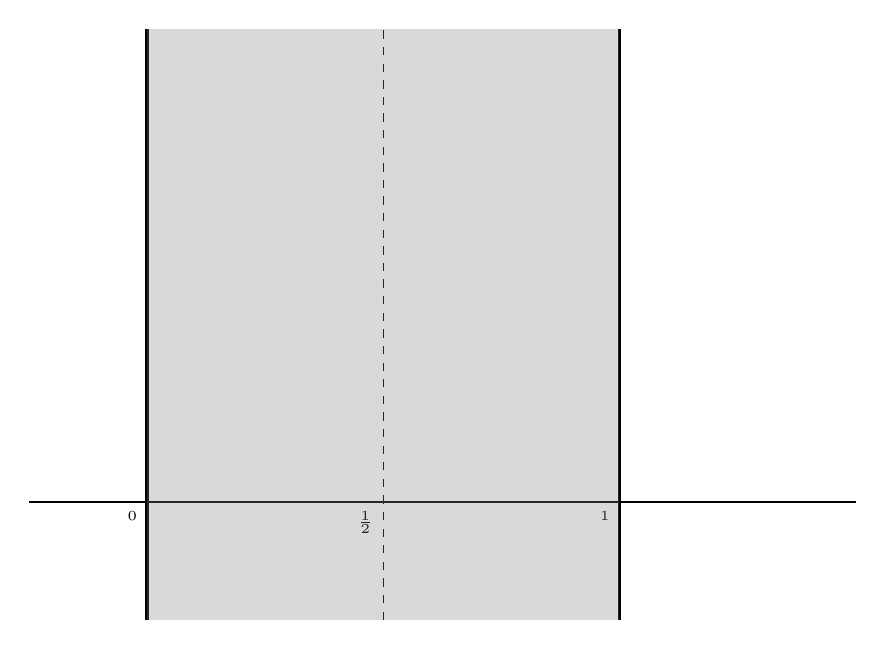
\begin{tikzpicture}[scale=3]
        \def\xmin{-0.5} \def\xmax{3}
        \def\ymin{-0.5} \def\ymax{2}
        \draw[thick] (\xmin,0) -- (\xmax,0);
        \draw[very thick] (0,\ymin) -- (0,\ymax);
        \draw[very thick] (2,\ymin) -- (2,\ymax);
        \draw[dashed] (1,\ymin) -- (1,\ymax);

        \node at (0,0) [below left] {\tiny{$0$}};
        \node at (1,0) [below left] {\tiny{$\frac{1}{2}$}};
        \node at (2,0) [below left] {\tiny{$1$}};

        \begin{scope}
          \path[clip] (0,\ymin) -- (0,\ymax) -- (2,\ymax) -- (2,\ymin) -- cycle;
          \fill[gray,opacity=0.3] (0,\ymin) rectangle (2,\ymax);
        \end{scope}
      \end{tikzpicture}
      \caption{The critical strip and critical line.}
      \label{fig:critical_strip}
    \end{figure}
  \section{The Approximate Functional Equation}
    If $L(s,f)$ is an $L$-function, then there is a formula which acts as a compromise between the functional equation for $L(s,f)$ and expressing $L(s,f)$ as a Dirichlet series. This formula is known as the approximate functional equation and it is important because it is valid inside of the critical strip and therefore can be used to obtain data about $L(s,f)$. First, we need to state an important asymptotic about the ratio of gamma factors that we will use later on. Let $s = \s+it$, $\s$ is bounded, and $|t| > 1$. This guarantees that $s$ is bounded away from zero. Recall
    \[
        \G(s) \sim \sqrt{2\pi}|t|^{\s-\frac{1}{2}}e^{-\frac{\pi}{2}|t|},
    \]
    which comes from \cref{equ:weaker_Stirling_formula}. This gives the weaker estimates
    \begin{equation}\label{equ:simplified_gamma_estimates}
      \G(s) \ll t^{\s-\frac{1}{2}}e^{-\frac{\pi}{2}|t|} \quad \text{and} \quad \frac{1}{\G(s)} \ll t^{\frac{1}{2}-\s}e^{\frac{\pi}{2}|t|} .
    \end{equation}
    We can use these estimates to that $L(s,f)$ is has polynomial growth in the $t$-aspect in vertical strips:

    \begin{proposition}\label{prop:L_function_bounded_in_vertical_strips}
      If $L(s,f)$ is an $L$-function, then for any real $a$ and $b$ with $a < b$ there is a real $\a$ such that
      \[
        L(s,f) \ll t^{\a},
      \]
      in the vertical strip
      \[
        \{s = \s+it \in \C:a \le \s \le b, |t| > 1\}.
      \]
    \end{proposition}
    \begin{proof}
      Let $\e > 0$. Since $L(s,f)$ is absolutely convergent for $\Re(s) > 1+\e$, $L(s,f) \ll_{\e} 1$ in this region. If $|t| > 1$ we are away from the possible poles of $L(s,f)$, so by the functional equation
      \[
        L(s,f) \ll \frac{\g(1-s,f)}{\g(s,f)}L(1-s,f).
      \]
      Using \cref{equ:simplified_gamma_estimates} and the definition of $\g(s,f)$, it follows that
      \[
        \frac{\g(1-s,f)}{\g(s,f)} \ll t^{\a(\s)},
      \]
      where $\a(\s)$ is a real-valued continuous function. Letting $\s < 0$ and noting that $L(1-s) \ll 1$, we have
      \[
        L(s,f) \ll t^{\a(\s)}.
      \]
      for $\Re(s) < 0$ and where $\a(\s)$ is real and depends upon $\s$. As $L(s,f)$ is holomorphic for $|t| > 1$ and of order $1$, we can apply the Phragm\'en-Lindel\"of convexity principle (see \cref{append:The_Phragmen_Lindelof_Convexity_principle}) so that the estimate
      \[
        L(s,f) \ll t^{\a(\s)},
      \]
      holds for all $s$ with $|t| > 1$. Restricting $a < \s < b$, $\a(\s)$ takes a maximum value on the compact set $[a,b]$ which completes the proof. 
    \end{proof}

    \cref{prop:L_function_bounded_in_vertical_strips} is a very important property that $L$-functions possess. It is usually used to estimate Perron type formulas. We can also use it to deduce the \textbf{approximate function equation}\index{approximate function equation}:

    \begin{theorem}[Approximate functional equation]
      Let $L(s,f)$ be an $L$-function and let $G(u)$ be an even holomorphic function bounded on the strip $|\Re(u)| < a$, for any $a > 1$, and such that $g(0) = 1$. Let $X > 0$. Then for $s$ in the critical strip,
      \[
        L(s,f) = \sum_{n \ge 1}\frac{a_{f}(n)}{n^{s}}V_{s}\left(\frac{n}{\sqrt{q(f)}X}\right)+\e(s,f)\sum_{n \ge 1}\frac{\conj{a_{f}(n)}}{n^{1-s}}V_{1-s}\left(\frac{nX}{\sqrt{q(f)}}\right)-\frac{R}{q^{\frac{s}{2}}\g(s,f)},
      \]
      where $V_{s}(y)$ is a smooth function defined by
      \[
        V_{s}(y) = \frac{1}{2\pi i}\int_{(a)}\frac{\g(s+u,f)}{\g(s,f)}G(u)y^{-u}\frac{du}{u},
      \]
      and
      \[
        \e(s,f) = \e(f)q(f)^{\frac{1}{2}-s}\frac{\g(1-s,f)}{\g(s,f)}.
      \]
      Moreover, the remainder $R$ is zero if $\L(s,f)$ is entire and otherwise
      \[
        R = \left(\Res_{u = 1-s}+\Res_{u = -s}\right)\frac{\L(s+u,f)G(u)X^{u}}{u}.
      \]
    \end{theorem}
    \begin{proof}
      Let
      \[
        I(X,s,f) = \frac{1}{2\pi i}\int_{(a)}\L(s+u,f)G(u)X^{u}\,\frac{du}{u}.
      \]
      By our choice of $a$ and that $s$ is in the critical strip, $\Re(s+u) > 1$ so that $L(s+u) \ll 1$. Moreover, from \cref{equ:weaker_Stirling_formula} we see that $\g(s+u,f)$ has exponential decay. Since $G(u)$ is bounded, it follows that the integral is absolutely bounded by \cref{met:decay_compacta_integral}. By \cref{prop:L_function_bounded_in_vertical_strips} and \cref{equ:weaker_Stirling_formula}, the integrand also had exponential decay in a vertical strip containing $|\Re(u)| \le a$. Therefore we may shift the line of integration to $(-a)$. We pass by a simple pole at $u = 0$ and possible poles at $u = 1-s$ and $u = -s$, giving
      \[
        I(X,s,f) = \frac{1}{2\pi i}\int_{(-a)}\L(s+u,f)G(u)X^{u}\,\frac{du}{u}+\L(s,f)+R.
      \]
      Applying the functional equation to $\L(s+u,f)$ and performing the change of variables $u \to -u$, we obtain
      \[
        I(X,s,f) = -\e(f)I(X^{-1},1-s,\conj{f})+\L(s,f)+R,
      \]
      since $G(u)$ is even. This equation is equivalent to
      \[
        \L(s,f) = I(X,s,f)+\e(f)I(X^{-1},1-s,\conj{f})-R.
      \]
      Since $\Re(s+u) > 1$, we can expand the $L$-function $L(s,f)$ inside of $I(X,s,f)$ as a Dirichlet series:
      \begin{align*}
        I(X,s,f) &= \frac{1}{2\pi i}\int_{(a)}\L(s+u,f)G(u)X^{u}\,\frac{du}{u} \\
        &= \frac{1}{2\pi i}\int_{(a)}q(f)^{\frac{s+u}{2}}\g(s+u,f)L(s+u,f)G(u)X^{u}\,\frac{du}{u} \\
        &= \frac{1}{2\pi i}\int_{(a)}\sum_{n \ge 1}\frac{a_{f}(n)}{n^{s+u}}q(f)^{\frac{s+u}{2}}\g(s+u,f)G(u)X^{u}\,\frac{du}{u} \\
        &= \sum_{n \ge 1}\frac{1}{2\pi i}\int_{(a)}\frac{a_{f}(n)}{n^{s+u}}q(f)^{\frac{s+u}{2}}\g(s+u,f)G(u)X^{u}\,\frac{du}{u} && \text{DCT} \\
        &= q(f)^{\frac{s}{2}}\g(s,f)\sum_{n \ge 1}\frac{a_{f}(n)}{n^{s}}\frac{1}{2\pi i}\int_{(a)}\frac{\g(s+u,f)}{\g(s,f)}G(u)\left(\frac{\sqrt{q(f)}X}{n}\right)^{u}\,\frac{du}{u} \\
        &= q(f)^{\frac{s}{2}}\g(s,f)\sum_{n \ge 1}\frac{a_{f}(n)}{n^{s}}V_{s}\left(\frac{n}{\sqrt{q(f)}X}\right).
      \end{align*}
      Performing the same computation for $I(X^{-1},1-s,\conj{f})$ and substituting in the results, we arrive at
      \[
        \L(s,f) = q(f)^{\frac{s}{2}}\g(s,f)\sum_{n \ge 1}\frac{a_{f}(n)}{n^{s}}V_{s}\left(\frac{n}{\sqrt{q(f)}X}\right)+\e(f)q(f)^{\frac{1-s}{2}}\g(1-s,f)\sum_{n \ge 1}\frac{a_{f}(n)}{n^{1-s}}V_{1-s}\left(\frac{nX}{\sqrt{q(f)}}\right)-R.
      \]
      Diving by $q^{\frac{s}{2}}\g(s,f)$ completes the proof.
    \end{proof}

    The idea of the approximate functional equation was developed by Hardy and Littlewood in the series \cite{hardyzeros1921,hardyapproximate1923,hardyapproximate1929}.

    \begin{remark}\label{rem:effect_of_V_in_approximate_functional_equation}
      The function $V_{s}\left(y\right)$ has the effect of smoothing out the two sums in the right-hand side of the approximate functional equation. Indeed, this function restricts the sums to $n \ll \sqrt{q(f)}$ up to some error. For if $\frac{n}{\sqrt{q(f)}X} \ll 1$ we see that
      \[
        V_{s}\left(\frac{n}{\sqrt{q(f)}X}\right) \ll 1,
      \]
      for this range of $n$. For $n \gg \sqrt{q(f)}$, the integrand of $V_{s}\left(\frac{n}{\sqrt{q(f)}X}\right)$ has exponential decay coming from the $\left(\frac{n}{\sqrt{q(f)}X}\right)^{-u}$ factor as the ratio of gamma factors has polynomial growth by \cref{equ:simplified_gamma_estimates} and $G(u)$ is bounded by assumption. As $s$ is in the critical strip, the exact same estimates hold for $V_{1-s}\left(\frac{n}{\sqrt{q(f)}X}\right)$.
    \end{remark}
  \section{The Riemann Hypothesis \& Nontrivial Zeros}
    The zeros of $L$-functions $L(s,f)$ are closely tied to important arithmetic data of $f$. Let $L(s,f)$ be a degree $d$ $L$-function so that
    \[
      L(s,f) = \prod_{p}(1-\a_{1}(p)p^{-s})^{-1}(1-\a_{2}(p)p^{-s})^{-1} \cdots (1-\a_{d}(p)p^{-s})^{-1},
    \]
    for $\Re(s) > 1$. This product vanishes if and only if one of its factors are zero. As $\Re(s) > 1$, this is impossible so that $L(s,f)$ has no zeros in this region. The functional equation will allow us to understand more about the zeros of $L(s,f)$. Rewrite the functional equation for $L(s,f)$ as
    \begin{equation}\label{equ:fun_eq_for_zeros}
      L(s,f) = \e(f)q(f)^{\frac{1}{2}-s}\frac{\g(1-s,f)}{\g(s,f)}L(1-s,\conj{f}).
    \end{equation}
    If $\Re(s) < 0$ then $L(1-s,\conj{f})$ is nonzero by our previous comments. Moreover, $\g(1-s,f)$ is holomorphic in this region because $\Re(\k_{i}) \ge -1$ for all $i$. We conclude that poles of $\g(s,f)$ are zeros of $L(s,f)$ for $\Re(s) < 0$. Such zeros are called \textbf{trivial zeros}\index{trivial zeros}. From the definition of $\g(s,f)$, they are all simple and are of the form $s = \k_{i}-2n$ for some local root at infinity $\k_{i}$ and some integer $n \ge 0$. Any other zero of $L(s,f)$ is called a \textbf{nontrivial zeros}\index{nontrivial zeros} and it lies inside of the critical strip.

    \begin{remark}\label{rem:poles_of_completed_L_function}
      Recall that for any $L$-function $L(s,f)$, the completed $L$-function $\L(s,f)$ is required to be meromorphic on $\C$ with at most poles at $s = 0$ and $s = 1$. We have shown that the trivial zeros of $L(s,f)$ are poles of $\g(s,f)$ for $\Re(s) < 0$ and they are all simple. As $L(s,f)$ is meromorphic on $\C$ with at most a pole at $s = 1$, and $\g(s,f)$ has at most a pole at $s = 0$ for $\Re(s) \ge 0$, $\L(s,f)$ is meromorphic on $\C$ with at most poles at $s = 0$ and $s = 1$.
    \end{remark}
    
    Now let $\rho$ be a nontrivial zero of $L(s,f)$. Note that $\conj{L(s,f)} = L(\conj{s},\conj{f})$ by the identity theorem and that this equality holds for $\Re(s) > 1$ where $L(s,f)$ is defined by a Dirichlet series. It follows that $\conj{\rho}$ is a nontrivial zero of $L(s,\conj{f})$. In the interior of critical strip, the gamma factor is nonzero and holomorphic (again we have used $\Re(\k_{i}) \ge 1$ for all $i$). From the functional equation, it follows that $1-\conj{\rho}$ is also a nontrivial zero of $L(s,f)$. In short, the nontrivial zeros occur in pairs:
    \[
      \rho \quad \text{and} \quad 1-\conj{\rho}.
    \]
    We can sometimes say more. If $L(s,f)$ takes real values for real $s > 1$, the Schwarz reflection principle implies $L(\conj{s},f) = \conj{L(s,f)}$ and that $L(s,f)$ takes real values on the entire real axis save for the possible poles at $s = 0$ and $ s = 1$. We find that $\conj{\rho}$ and $1-\conj{\rho}$ are nontrivial zeros too and therefore the nontrivial zeros of $L(s,f)$ come in sets of four:
    \[
      \rho, \quad \conj{\rho}, \quad 1-\rho, \quad \text{and} \quad 1-\conj{\rho}.
    \]
    The \textbf{(Selberg class) Riemann hypothesis}\index{(Selberg class) Riemann hypothesis} says that this symmetry should be as simple as possible:

    \begin{conjecture}[Riemann hypothesis, Selberg class version]
      All of the nontrivial zeros of any $L$-function $L(s,f)$ belonging to the Selberg class lie on the line $\Re(s) = \frac{1}{2}$.
    \end{conjecture}
  \section{The Lindel\"of Hypothesis \& Convexity Arguments}
    Instead of asking about the zeros of an $L$-function $L(s,f)$ on the critical line, we can ask about the growth of $L(s,f)$ on the critical line. A \textbf{convexity argument}\index{convexity argument} is one where estimates about the growth of an $L$-function on the critical line are deduced. Usually this is achieved by methods of complex analysis and Sirling's formula. The standard argument for any $L$-function is known \textbf{Lindel\"of convexity argument}\index{Lindel\"of convexity argument}. It is essentially a refinement of the proof of \cref{prop:L_function_bounded_in_vertical_strips}. Suppose $L(s,f)$ has a degree $d$ Euler product. Also suppose $L(s,f)$ as a pole of order $r \ge 0$ at $s = 1$ and let
    \[
      p_{r}(s) = \left(\frac{s-1}{s+1}\right)^{r}.
    \]
    Note that $p_{r}(s) \sim 1$. The first step is to guarantee the Phragm\'en-Lindel\"of convexity principle for $p_{r}(s)L(s,f)$ in a region containing the critical strip. As $L(s,f)$ is of order $1$, this is assured (see \cref{append:The_Phragmen_Lindelof_Convexity_principle}). Therefore, we are reduced to estimating the growth of $p_{r}(s)L(s,f)$ for $\s$ to the left of $0$ and to the right of $1$. That is, just outside the edges of the critical strip. So we will assume $-\e \le \s \le 1+\e$ for some $\e > 0$. The right edge is easily estimated by setting $\s = 1+\e$ so that
    \begin{equation}\label{equ:convexity_bound_1}
      p_{r}(1+\e+it)L(1+\e+it,f) \ll_{\e} 1.
    \end{equation}
    The left edge is only slightly more difficult. The functional equation implies
    \begin{equation}\label{equ:convexity_bound_left_edge}
      p_{r}(s)L(s,f) \ll \frac{\g(1-s,f)}{\g(s,f)}p_{r}(s)L(1-s,f).
    \end{equation}
    From \cref{equ:simplified_gamma_estimates}, the definition of $\g(s,f)$, and that $L(s,f)$ has $d$ gamma functions in its gamma factor, it follows that
    \[
      \frac{\g(1-s,f)}{\g(s,f)} \ll (q(f)t^{d})^{\frac{1-2\s}{2}},
    \]
    for $-\e \le \s \le 1+\e$ with $|t| > 1$. Since the region
    \[
      \{s = \s+it \in \C:-\e \le \s \le 1+\e,|t| \le 1\},
    \]
    is compact and $q\left(s,f\right) \sim q(f)t^{d}$ for $-\e \le \s \le 1+\e$, we have the improved estimate
    \begin{equation}\label{equ:ratio_gamma_factor_explicit}
      \frac{\g(1-s,f)}{\g(s,f)} \ll q(s,f)^{\frac{1-2\s}{2}},
    \end{equation}
    for $-\e \le \s \le 1+\e$. Setting $\s = -\e$ and combining \cref{equ:convexity_bound_1,equ:convexity_bound_left_edge,equ:ratio_gamma_factor_explicit} gives
    \begin{equation}\label{equ:convexity_bound_2}
      p_{r}(-\e+it)L(-\e+it,f) \ll_{\e} q(s,f)^{\frac{1}{2}+\e}.
    \end{equation}
    By the Phragm\'en-Lindel\"of convexity principle, \cref{equ:convexity_bound_1,equ:convexity_bound_2}, and that $p_{r}(s) \sim 1$, we obtain
    \[
      L(s,f) \ll_{\e} q(s,f)^{\frac{1+\e-\s}{2}},
    \]
    for $-\e \le \s \le 1+\e$. At the critical line, we have the \textbf{convexity bound}\index{convexity bound}:
    \begin{equation}\label{equ:convexity_bound_L_function}
      L\left(\frac{1}{2}+it,f\right) \ll_{\e} q\left(\frac{1}{2}+it,f\right)^{\frac{1}{4}+\e}.
    \end{equation}
    The \textbf{(Selberg class) Lindel\"of hypothesis}\index{(Selberg class) Lindel\"of hypothesis} says that the exponent can be reduced to $\e$:

    \begin{conjecture}[Lindel\"of hypothesis, Selberg class version]
      For any $L$-function $L(s,f)$ belonging to the Selberg class and any $\e > 0$,
      \[
        L\left(\frac{1}{2}+it,f\right) \ll_{\e} q\left(\frac{1}{2}+it,f\right)^{\e}.
      \]
    \end{conjecture}

    For any $L$-function $L(s,f)$, any improvement upon the exponent in the convexity bound in any aspect of the analytic conductor is called \textbf{breaking convexity}\index{breaking convexity} (or a \textbf{convexity breaking bound}\index{convexity breaking bound}). Any argument used to do so is called a \textbf{subconvexity argument}\index{subconvexity argument}.